\documentclass[convert]{standalone}

\usepackage{tikz}
\usepackage{graphicx}
\pagestyle{empty}

% INT_AY22_L28-Fig16_Changing_fields.png

\begin{document}
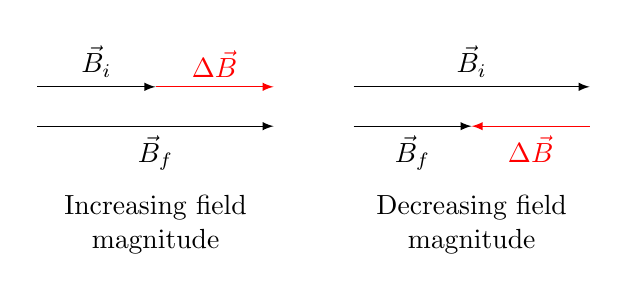
\begin{tikzpicture}[> = latex]
\matrix[column sep = 1 cm]{

	% Increasing field
	
	\draw [->] (0, 0.25) -- node [above] {${\vec B}_i$} (1.5, 0.25);
	\draw [->] (0, -0.25) -- node [below] {${\vec B}_f$} (3, -0.25);
	
	% Change in field
	
	\draw [->, red] (1.5, 0.25) -- node [above] {$\Delta {\vec B}$} (3, 0.25);
	
	% Label change
	
	\node [align = center] at (1.5, -1.5) {Increasing field\\magnitude};
	
&

	% Decreasing field
	
	\draw [->] (0, 0.25) -- node [above] {${\vec B}_i$} (3, 0.25);
	\draw [->] (0, -0.25) -- node [below] {${\vec B}_f$} (1.5, -0.25);
	
	% Change in field
	
	\draw [->, red] (3, -0.25) -- node [below] {$\Delta {\vec B}$} (1.5, -0.25);
	
	% Label change
	
	\node [align = center] at (1.5, -1.5) {Decreasing field\\magnitude};

\\
};
\end{tikzpicture}
\end{document}